\documentclass[11pts]{report}

\usepackage{qtree}
\usepackage{listings}
\usepackage{amsmath,mathtools}
\usepackage[ruled,longend]{algorithm2e}
\usepackage{tikz}
\usepackage{listings}
\usepackage{graphicx}
\usepackage{xcolor}
\usepackage{array}
\lstset{
    frame=tb, % draw a frame at the top and bottom of the code block
    tabsize=4, % tab space width
    showstringspaces=false, % don't mark spaces in strings
    commentstyle=\color{green}, % comment color
    keywordstyle=\color{blue}, % keyword color
    stringstyle=\color{red} % string color
}

\title{CS 677 Homework \\ Assignment 07}
\author{\textbf{Hai Nguyen}}

\setlength{\topmargin}{-1cm}
\setlength{\oddsidemargin}{0in}
\setlength{\textwidth}{6.5in}
\setlength{\textheight}{8.3in}

\DeclareMathOperator{\Div}{div}
\newcommand{\vect}[1]{\mathbf{#1}}




%%Currently default settings for indentation and symbols.
%%Try these by uncommenting this block!!!
%%Redefine the first level symbols
%\renewcommand{\theenumi}{\fnsymbol{enumi}-}
%\renewcommand{\labelenumi}{\theenumi}
%
%%Redefine the second level symbols
%\renewcommand{\theenumii}{\alph{enumii})}
%\renewcommand{\labelenumii}{\theenumii}
%
%%Redefine the third level symbols
%\renewcommand{\theenumiii}{\roman{enumiii}.}
%\renewcommand{\labelenumiii}{\theenumiii}
%
%%Options for redefining levels


%\arabic
%\alph 
%\Alph
%\roman
%\Roman
%\fnsymbol
%This ^^^ is all you need to change!!

\begin{document}

\maketitle

\begin{enumerate}

% Question 1
\item 
\textit{Greedy strategy:}
\begin{itemize}
\item Order works based on their weight per time

\begin{equation*}
\frac{w_1}{t_1} \geq \frac{w_2}{t_2} \geq \hdots \geq \frac{w_n}{t_n}
\end{equation*}

\item Pick the work with the smaller weight per time $\frac{w_i}{t_i}$ to perform first

\end{itemize}


\begin{figure}[htbp]
\begin{center}
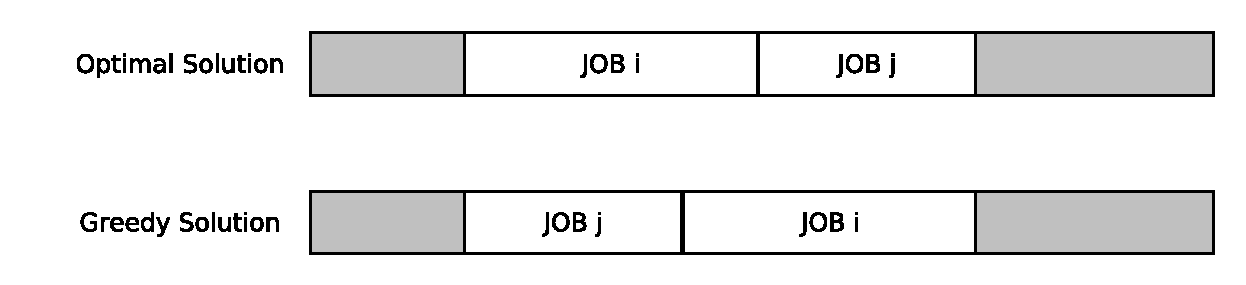
\includegraphics[scale=0.5]{Q_1.pdf}
\caption{Compare optimal and greedy solution.}
\label{Fig:1}
\end{center}
\end{figure}

\textit{Prove greedy choice property:}


Assume that we are given an optimal solution as in Figure \ref{Fig:1}, we prove that by using the greedy choice, we can come up with a better or equal solution. For the optimal solution, there should be no gap between jobs.

As the optimal solution does not follow the greedy choice (if it follows then we are done), we have:

\begin{equation}
\frac{w_i}{t_i} \geq \frac{w_j}{t_j}
\label{eq1}
\end{equation}

The weighted sum of completion time is:
\begin{equation*}
S_{opt} = S_{i^-} + (C+ t_i) \times w_i + (C + t_i + t_j) \times w_j + S_{j^+}
\end{equation*}
With $S_{i^-}$ is the weighted sum of jobs scheduled before job i and $S_{j^+}$ is the weighted sum of jobs scheduled after job j. $C$ is the finishing time of jobs earlier than $i$ and $j$.
Assume that we use our greedy choice and pick job j to do first as it has smaller weight per time. The weighted sum of completion time is:
\begin{equation*}
S_{gred} = S_{i^-} + (C + t_j) \times w_j + (C + t_j + t_i) \times w_i + S_{j^+}
\end{equation*}

However from (\ref{eq1}), we have:
\begin{equation*}
S_{gred} - S{opt} = t_j \times w_i - t_i \times w_j \geq 0
\end{equation*}

Therefore, by using greedy choice we always find an equal or better solution than the optimal solution.

\item \textit{Greedy strategy:}

\begin{itemize}
\item Begin from the shift $S_1$ that starts the earliest, pick the worker who do the longest shift from the list of all shifts that overlapps with $S_1$ to form the advisory committee.
\item When done with $S_1$, continue with the next shift that starts earliest after the shift of the above selected worker and perform the same strategy to choose the next worker for the committee.
\end{itemize}

\textit{Prove greedy choice property:}
Assume that we are given a optimal solution for the advisory committee. From this committee, for shift $S_i$, assume it is observed by a worker $w_j$ in the committee. From the definition of the committee, the shift that this worker takes  $S_j$ will overlap with the shift $S_i$. By using the greedy choice, we prove that we can have an equal or better solution.
\begin{itemize}
\item We know that $S_j$ will belong to a set of shifts that overlaps with shift $i$. When we replace $S_j$ by the greedy choice (the longest shift in the overlapped set), the new shift will of course satisfy the overllaping condition. 
\item However, the number of workers will be smaller or equal than that of the current committee as this new shift is the longest one therefore it has higher chance to overlap with other tasks than the previous selection of shift.
\item Therefore, by using the greedy choice and given an optimal choice of the committee, we can always construct a new advisory committee which is a complete but might contain fewer workers than the given committee.
\end{itemize}  

\item Construct an optimal Huffman coding tree for the characters I with frequency 75, U with frequency 200, B with frequency 25, S with frequency 275, C with frequency 50, H with
frequency 100, M with frequency 25, and P with frequency 250. How many bits are required to store the above characters using the resulting encoding.

\begin{center}
 \begin{tabular}{|c | c c c c c c c c|} 
 \hline
 Letter & I & U & B & S & C & H & M & P \\ 
 \hline
 Freq. & 75 & 200 & 25 & 275 & 50 & 100 & 25 & 250 \\ 
 \hline
\end{tabular}
\end{center}


\begin{figure}[htbp]
\begin{center}
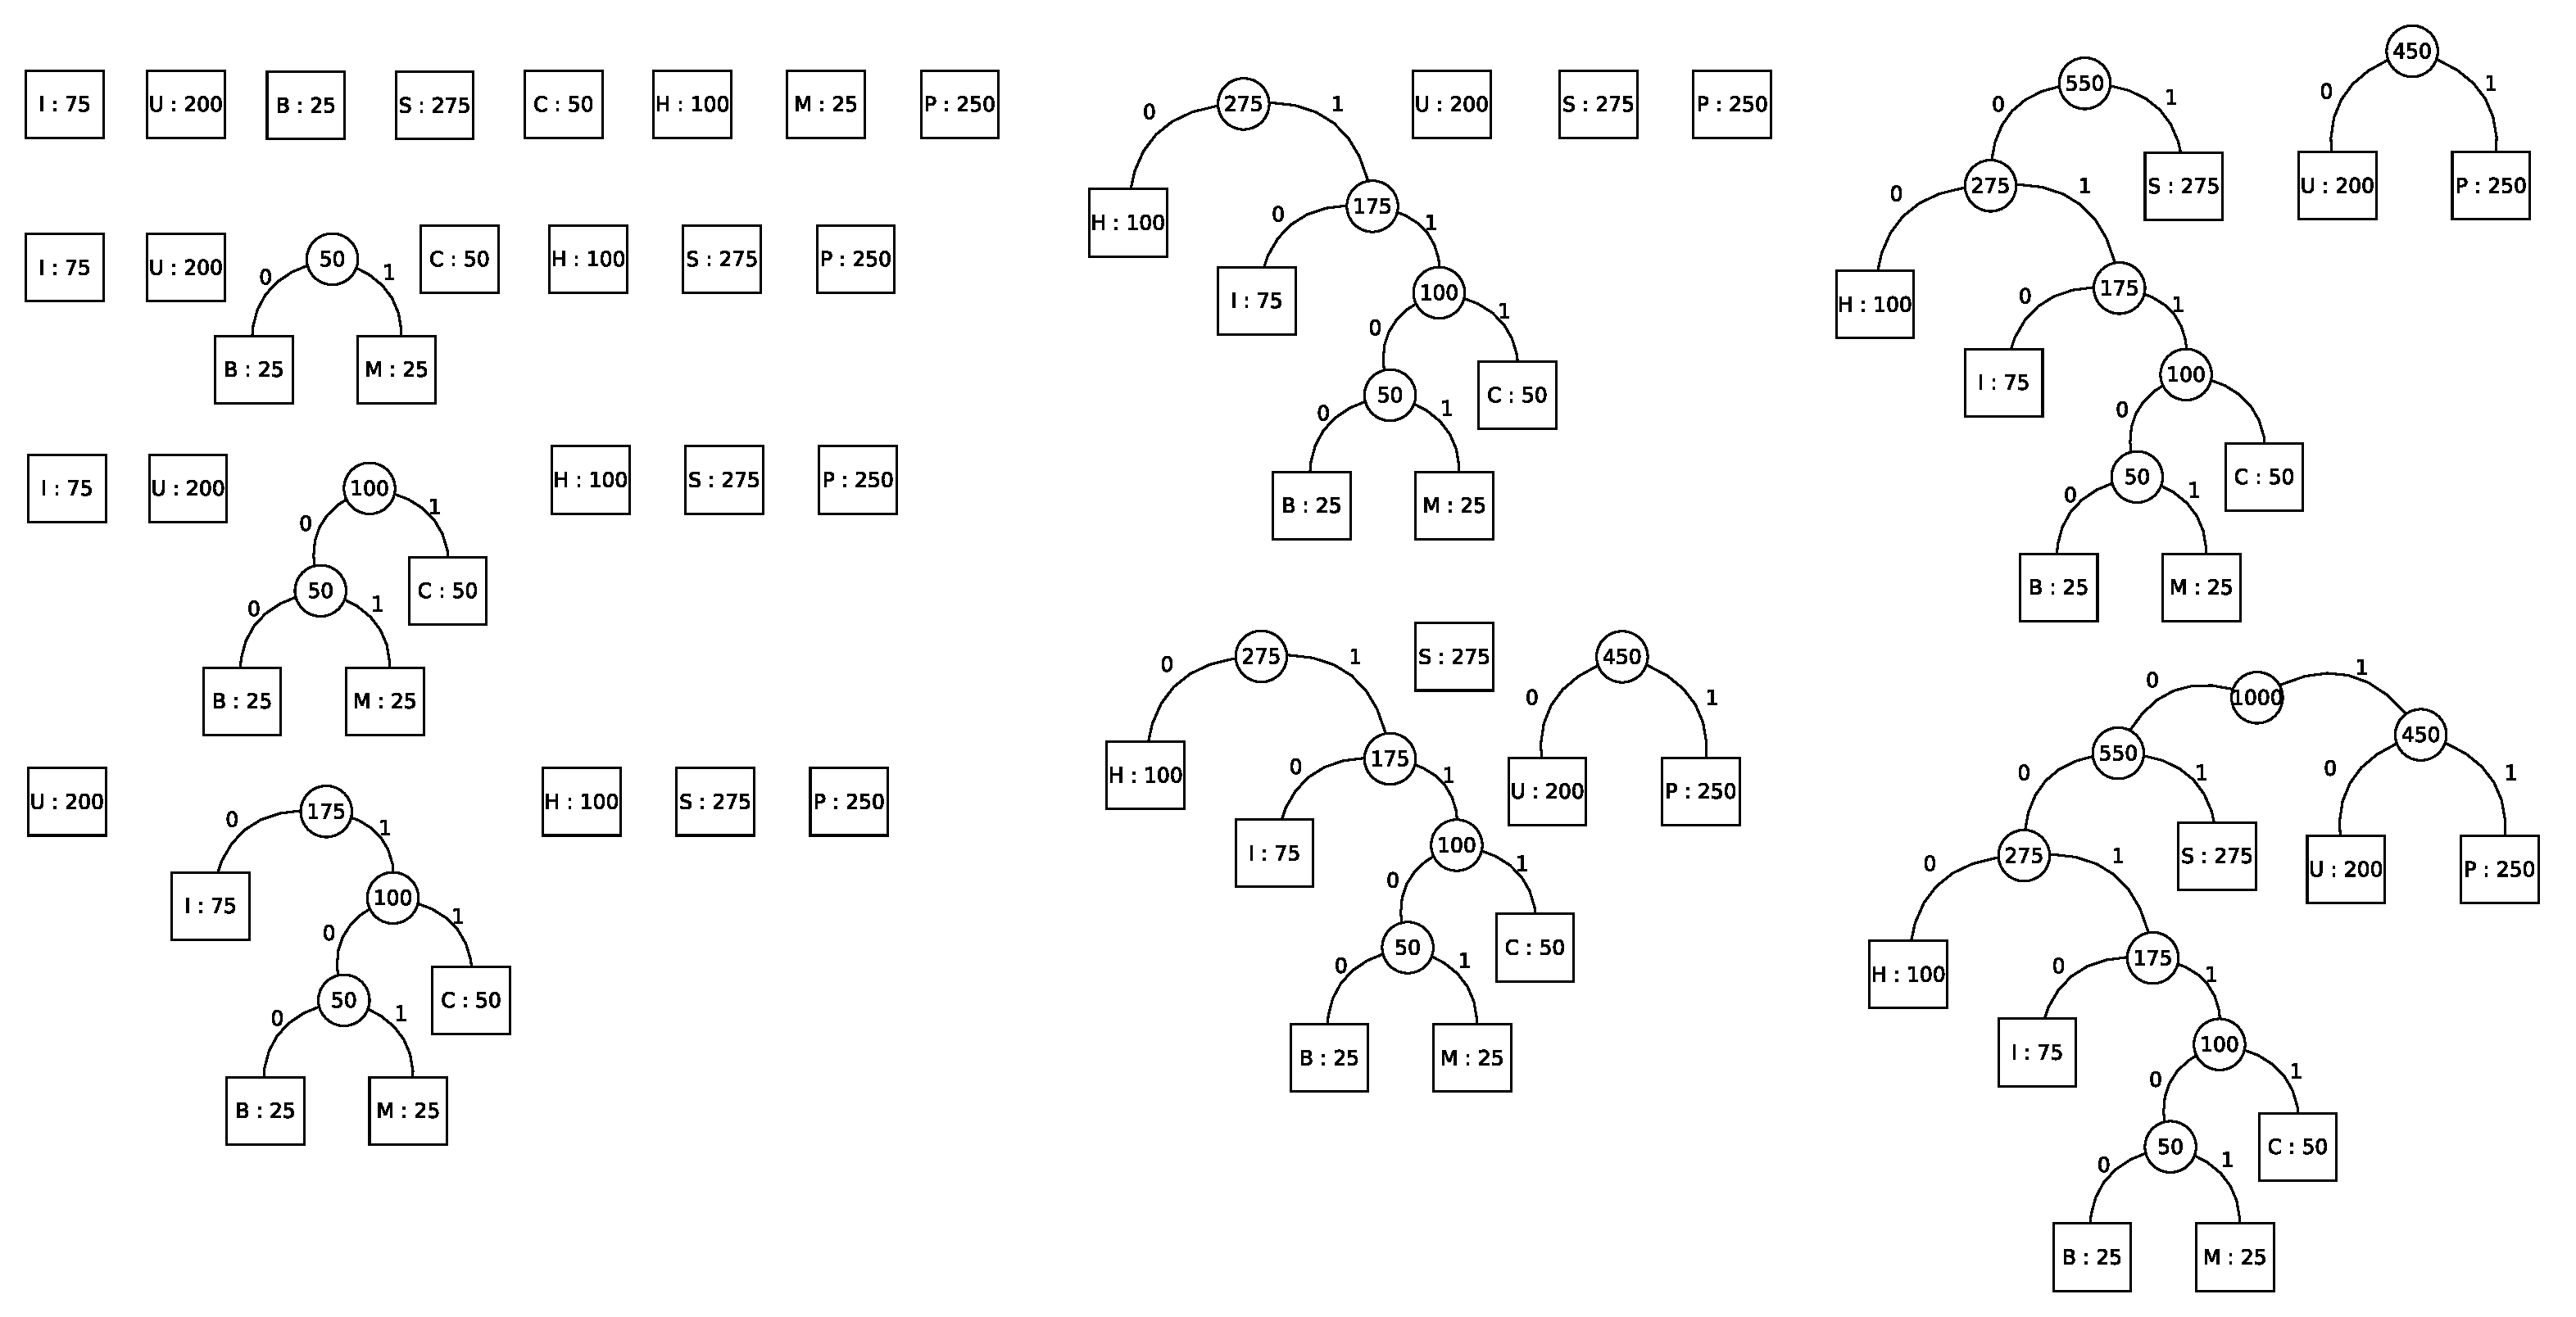
\includegraphics[scale=0.32]{1.pdf}
\caption{Construct a Huffman code.}
\label{Fig:1a}
\end{center}
\end{figure}

Based on Figure \ref{Fig:1a}, the number of bits needed to store the characters:
\begin{equation*}
200 \times 2 + 100 \times 3 + 75 \times 4 + 25 \times 6 + 25 \times 6 + 250 \times 2 + 275 \times 2 + 50 \times  5 = 2600 \text{ (bits)}
\end{equation*}

\item If we use Huffman code, it is constructed as in Figure \ref{Fig:4}.
The total number of bits to encode is:
\begin{equation*}
6 \times 2 + 2 \times 4 + 3 \times 3 + 2 \times 4 + 8 \times 1 = 45 \text{ (bits)}
\end{equation*}


\begin{figure}[htbp]
\begin{center}
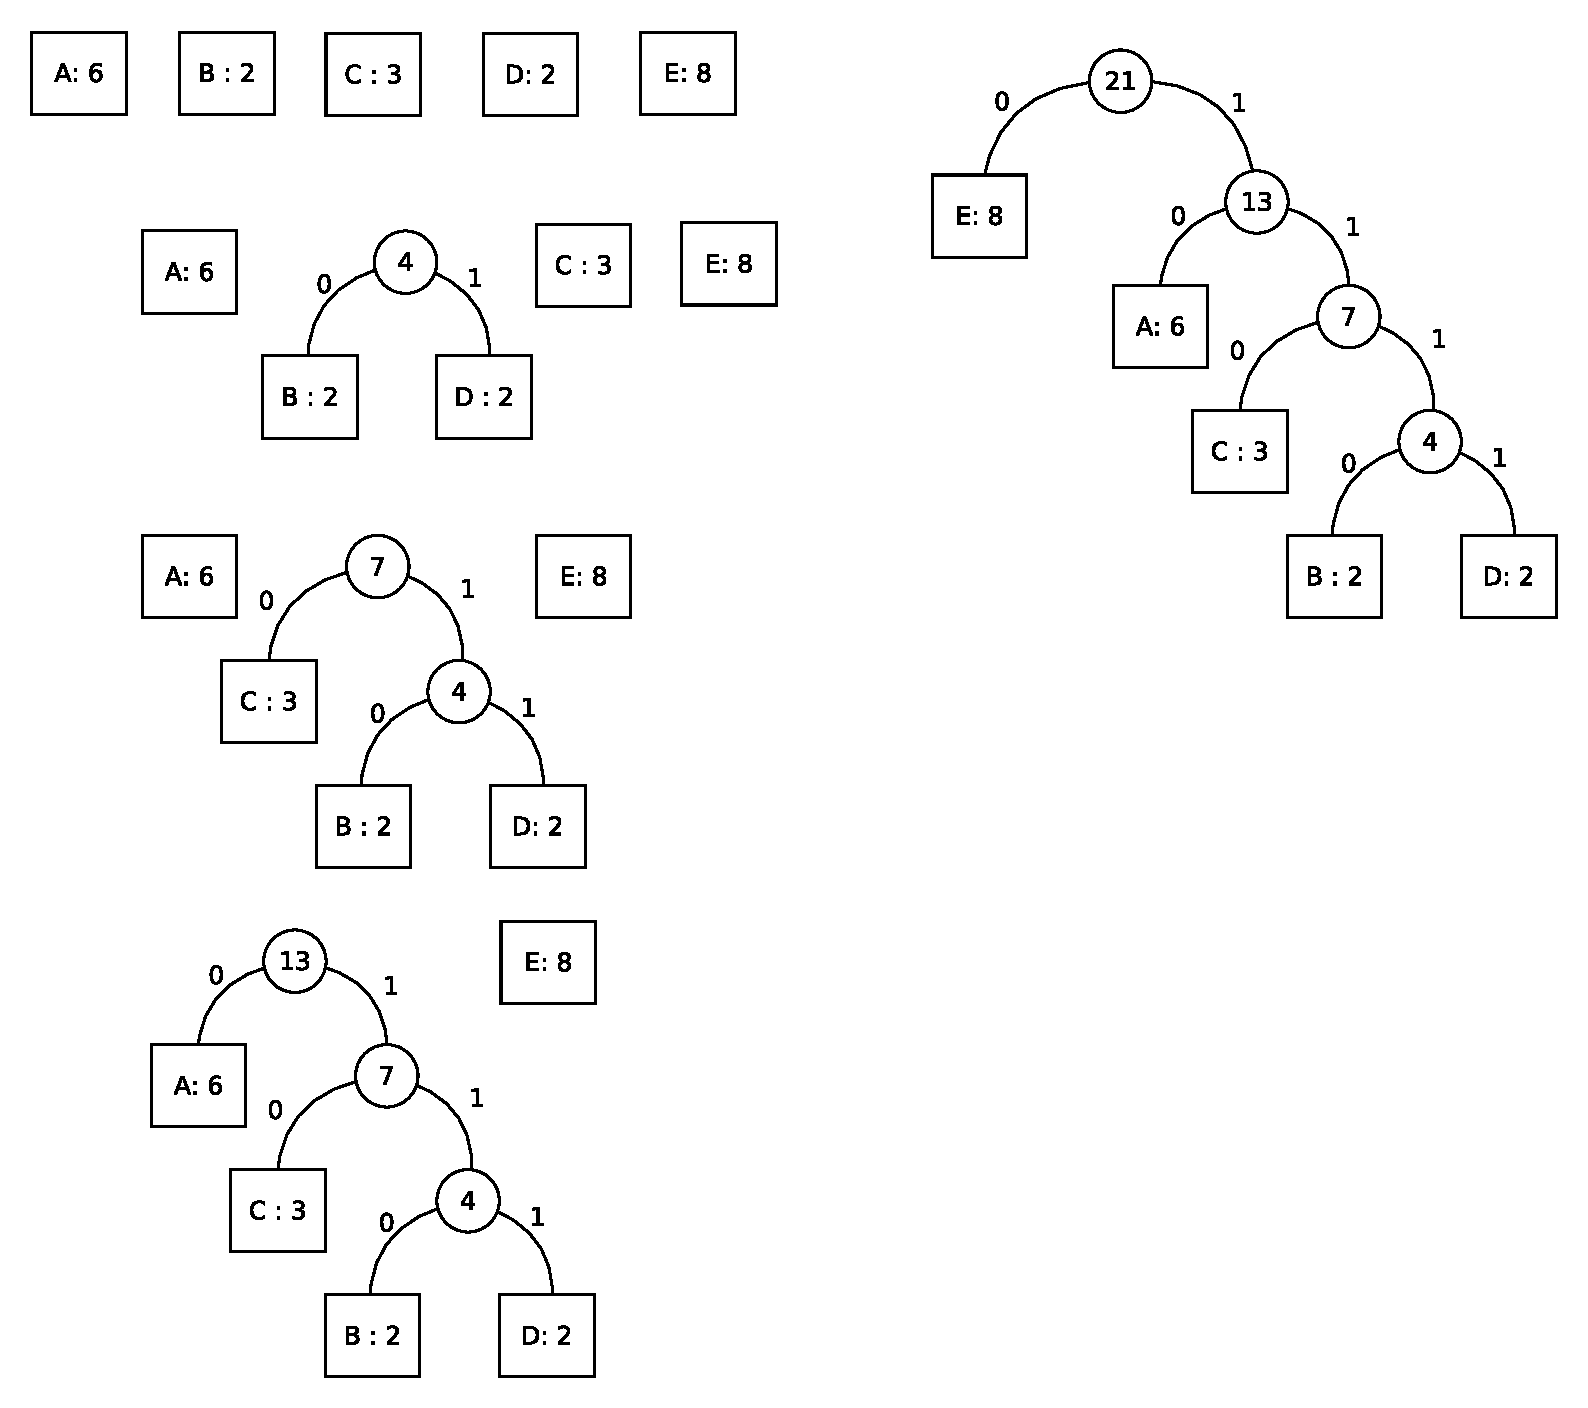
\includegraphics[scale=0.32]{4.pdf}
\caption{Construct Huffman code.}
\label{Fig:4}
\end{center}
\end{figure}

If using the suggestion from Professor Byte, the total number of bit is:
\begin{equation*}
6 \times 1 + 2 \times 2 + 3 \times 2 + 2 \times 2 + 8 \times 1 = 28 \text{ (bits)}
\end{equation*}

Therefore, to store the text, Professor Byte will use less space than using an optimal Huffman code. However, as the code suggested by Professor Byte are non-prefix codes, he will suffer from ambiguity when decoding the text. For instance, if there are pairs of text which encoded the same such as [AE D] = [100], [C EA] = [01] or [B EE] = [00]. Therefore, if the text does not contain ambiguous pairs of text like those are just mentioned, Professor Byte can use his code to encode and decode the text without any problem and it actually uses less space than using the optimal Huffman code.

\begin{figure}[htbp]
\begin{center}
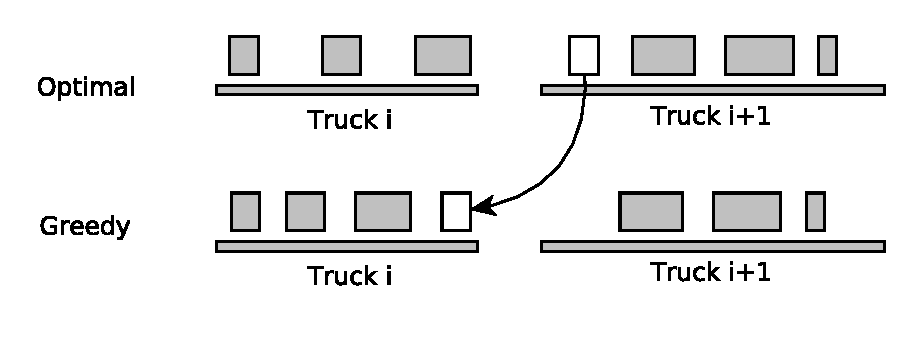
\includegraphics[scale=0.7]{5.pdf}
\caption{Package redistribution.}
\label{Fig:5}
\end{center}
\end{figure}

\item Assume that we are given an optimal strategy to minimize the number of trucks needed and the strategy does not use the current greedy policy. Thefore, at least one truck can still carry one more package (the first package of the next truck) - the white package as shown in Figure \ref{Fig:5}.




Thefore, we can redistribute the packages by using the given greedy strategy and move the white package back to the truck $i$. The current package distribution:

\begin{itemize}
\item Maintain the same or fewer number of trucks needed. The fewer case happens when the truck $i+1$ only contains the white package which is now carried by the truck $i$ therefore the truck $i+1$ is no longer needed.
\item All packages are still carried to the destination according to the order they are received.
\end{itemize}

Therefore, we can modify the given optimal solution to the same or even better solution by using the greedy strategy so that the packages carried by each truck will follow the greedy strategy. We then can conclude that the greedy strategy minimizes the number of trucks that are needed.

\end{enumerate}

\end{document}
